\documentclass[tikz,border=2pt]{standalone}
\usepackage{amsmath,amssymb}
\usepackage{xcolor}
\usetikzlibrary{positioning}
\begin{document}
% Extracted from namuenofull.inc; source column: \footnotesize \cite{NU}$_{\rm p{ 174 }}$ I$^*_{n}$-II$^*$-$\alpha$
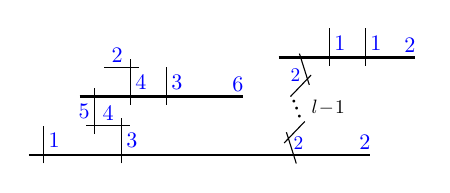
\begin{tikzpicture}[xscale=0.57,yscale=0.62]
\draw[thick,shorten >=2] (-1/3,0)--(37/5,0) node[inner sep=2pt,blue,above left,scale=0.8] {2} node[inner sep=2pt,below left,scale=0.8] {};
\draw[shorten <=-3pt] (0,0)--node[inner sep=2pt,scale=0.8,blue,right] {1} (0,3/5);
\draw[shorten <=-3pt, shorten >=-3pt] (26/15,0)--node[inner sep=2pt,scale=0.8,blue,right] {3} (26/15,3/5);
\draw[shorten <=-3pt, shorten >=-3pt] (26/15,3/5)--node[inner sep=2pt,scale=0.8,blue,above] {4} (17/15,3/5);
\draw[shorten <=-3pt, shorten >=-3pt] (17/15,3/5)--node[inner sep=2pt,scale=0.8,blue,left] {5} (17/15,6/5);
\draw[thick,shorten >=2] (4/5,6/5)--(137/30,6/5) node[inner sep=2pt,blue,above left,scale=0.8] {6} node[inner sep=2pt,below left,scale=0.8] {};
\draw[shorten <=-3pt, shorten >=-3pt] (29/15,6/5)--node[inner sep=2pt,scale=0.8,blue,right] {4} (29/15,9/5);
\draw[shorten <=-3pt] (29/15,9/5)--node[inner sep=2pt,scale=0.8,blue,above] {2} (4/3,9/5);
\draw[shorten <=-3pt] (41/15,6/5)--node[inner sep=2pt,scale=0.8,blue,right] {3} (41/15,9/5);
\draw (167/30,0) 
    ++(0.06,-0.17)--++(-0.22,0.64)++(0.11,-0.24)  
    ++(0,0.02)
      node[blue,scale=0.7,inner sep=1,anchor=west]{2}
    ++(0,-0.02)
    ++(-0.16,0.02)--++(0.46,0.44)++(-0.12,0.08)  
    node{$\cdot$} ++(-0.06,0.16) node{$\cdot$}
    ++(-0.06,0.16) node{$\cdot$}++(0.17,-0.12)    node[auto,inner sep=5,scale=0.7,anchor=west]{$l\!-\!1$}
    ++(-0.25,0.23)--++(0.46,0.44)++(-0.19,0.04)   
    ++(0,-0.05)
      node[blue,scale=0.7,inner sep=1,anchor=east]{2}
    ++(0,0.05)
    ++(0.19,-0.04)++(-0.04,-0.2)--++(-0.22,0.64);
\draw[thick,shorten >=2] (157/30,2)--(42/5,2) node[inner sep=2pt,blue,above left,scale=0.8] {2};
\draw[shorten <=-3pt] (191/30,2)--node[inner sep=2pt,scale=0.8,blue,right] {1} (191/30,13/5);
\draw[shorten <=-3pt] (43/6,2)--node[inner sep=2pt,scale=0.8,blue,right] {1} (43/6,13/5);
\end{tikzpicture}
\end{document}
